\newlength\cyclerad
\pgfmathsetlength{\cyclerad}{2cm}
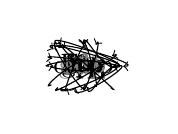
\begin{tikzpicture}
  \node[] at (0:\cyclerad) (atp) {atp};
  \node[gray] at (350:1.5*\cyclerad) (gluc) {gluc};
  \node[gray] at (330:1.5*\cyclerad) (adp1) {adp};
  \node[] at (320:\cyclerad) (g6p) {g6p};
  \node[] at (280:\cyclerad) (f6p) {f6p};
  \node[] at (235:\cyclerad) (fbp) {fbp};
  \node[gray] at (250:1.5*\cyclerad) (adp2) {adp};
  \node[] at (200:1.5*\cyclerad) (dhap) {dhap};
  \node[] at (180:\cyclerad) (gap) {gap};
  \node[gray] at (170:1.5*\cyclerad) (pi) {p};
  \node[] at (135:\cyclerad) (bpg) {bpg};
  \node[gray] at (120:1.5*\cyclerad) (adp3) {adp};
  \node[] at (100:\cyclerad) (3pg) {3pg};
  \node[] at (65:\cyclerad) (2pg) {2pg};
  \node[] at (30:\cyclerad) (pep) {pep};
  \node[gray] at (25:1.5*\cyclerad) (adp4) {adp};
  \node[gray] at (7:1.5*\cyclerad) (pyr) {pyr};
  \draw[->] (atp) [out=-135,in=0] to node [pos=0.9,shape=coordinate] (midpfk) {} (fbp);
  \draw[] (f6p) [out=140,in=0] to (midpfk);
  \draw[->] (midpfk) [out=190,in=90] to (adp2);
  \draw[->] (g6p) [out=220,in=20] to (f6p);
  \draw[->] (atp) [out=-90,in=60] to node [pos=0.5,shape=coordinate] (midpts) {} (g6p);
  \draw[] (gluc) [out=180,in=60] to (midpts);
  \draw[->] (midpts) [out=240] to (adp1);
  \draw[->] (fbp) [out=140,in=-85]to node [pos=0.3,shape=coordinate] (midfba) {} (gap) ;
  \draw[->] (midfba) [out=135,in=0] to (dhap);
  \draw[->] (dhap) -- (gap);
  \draw[->] (gap) [out=85,in=235] to node [pos=0.5,shape=coordinate] (mid3pg) {} (bpg) ;
  \draw[] (pi) [out=0,in=240] to (mid3pg);
  \draw[->] (bpg) [out=0,in=150] to node [pos=0.07,shape=coordinate] (midbpg) {} (atp);
  \draw[] (adp3) [out=-80,in=170] to (midbpg);
  \draw[->] (midbpg) [out=10,in=250] to (3pg);
  \draw[->] (3pg)  [out=0,in=166] to (2pg);
  \draw[->] (2pg) [out=-38,in=135] to (pep);
  \draw[->] (pep) [out=-59,in=90] to node [pos=0.5,shape=coordinate] (midpck) {}(atp);
  \draw[] (adp4) [out=210,in=120] to (midpck);
  \draw[->] (midpck) [out=300,in=180] to (pyr);
 \end{tikzpicture}
